\documentclass[a4paper,10.5pt,fontset=none]{ctexart}

\usepackage{mathpazo}
\setmainfont{TeX Gyre Pagella}
\setCJKmainfont[BoldFont={Noto Serif CJK SC Bold}]{Noto Serif CJK SC}
\setCJKsansfont{Noto Sans CJK SC}
\linespread{1.3}

\usepackage[margin=2cm,top=1.6cm,bottom=1.8cm]{geometry}
\usepackage{graphicx}
\usepackage{amsmath,amssymb}
\usepackage{xcolor}
\usepackage{enumitem}
\usepackage{fancyhdr}
\usepackage[hidelinks]{hyperref}

\definecolor{ink}{HTML}{1A1A1A}
\definecolor{accent}{HTML}{1F4E79}
\definecolor{warm}{HTML}{B4532A}
\definecolor{quiet}{HTML}{80868B}
\definecolor{hair}{HTML}{D5D8DC}

\color{ink}
\setlist{nosep,leftmargin=1.5em,itemsep=0.35em}
\setlength{\parindent}{0pt}
\setlength{\parskip}{0.45em}
\pagestyle{fancy}
\fancyhf{}
\lhead{\footnotesize\color{quiet}Use It or Lose It? \textperiodcentered{} 逐页中文详解}
\rhead{\footnotesize\color{quiet}\thepage}
\renewcommand{\headrulewidth}{0pt}

\newcommand{\euro}{€}
\newcommand{\quiet}[1]{{\color{quiet}#1}}
\newcommand{\hl}[1]{{\color{accent}#1}}
\newcommand{\kicker}[1]{{\small\bfseries\color{accent}#1}}
% \slidepage{page in slides.pdf}{heading}
\newcommand{\slidepage}[2]{%
  \clearpage
  \kicker{#2}\par\smallskip
  {\centering\setlength{\fboxsep}{0pt}\color{hair}\fbox{\includegraphics[page=#1,width=0.92\textwidth]{../slides/slides.pdf}}\par}
  \medskip
}
\newcommand{\sub}[1]{\par\smallskip{\color{accent}\bfseries #1}\par}

\begin{document}

% ================= 封面 =================
{\color{accent}\rule{1.6cm}{1.2pt}}\par\medskip
{\fontsize{24}{30}\selectfont Use It or Lose It?}\par\smallskip
{\large\quiet{逐页中文详解}}\par\medskip
{\small Zheng Huang \textperiodcentered{} Topics of Central Banking \textperiodcentered{} 2026 年 10 月}

\vspace{0.4cm}
\kicker{结构}

正文 17 页讲一条核心故事；附录 7 页放文献、方案对比、推导、校准细节和一个扩展（逆周期上限）。

\vspace{0.8cm}
\kicker{这份文档怎么用}

每一页上方是英文幻灯片原样，下方是中文详解，通常分四部分：\hl{这一页的意思}、\hl{怎么看图}、\hl{关键概念}、\hl{和整个故事的关系}。它不是讲稿，而是帮助你自己彻底弄懂每一页：为什么这么说、数字从哪里来、被追问时背后的道理是什么。

\vspace{0.4cm}
\kicker{全篇要回答的问题}

数字欧元应不应该计息？如果应该，以什么形式计息？

\vspace{0.4cm}
\kicker{一句话答案}

分析表明：如果要让货币带上持有成本，连续贬值（即负利率）是比到期日更自然的形式；把数字欧元利率锁在零有代价，它会抬高利率下限；结合价格与数量的思路，可以得到“支付免费额度 + 额度以上贬值 + 危机上限”的结构。报告的目的不是给欧洲央行开药方，而是把这些取舍讲清楚。

\vspace{0.4cm}
\kicker{故事线（17 个标题的中文意思）}
\begin{enumerate}[leftmargin=2.2em,itemsep=0.2em]
  \item[2] 本报告沿着一个问题，从消费券一路讲到数字欧元的设计。
  \item[3] 央行创造的钱没人花，货币政策就失去抓手。
  \item[4] 利率无法降到零以下太多，因为现金永远是零利率。
  \item[5] 带到期日的消费券能让钱被花出去，这正是流动性陷阱需要的。
  \item[6] 可编程的数字欧元可以把这种压力写进货币本身，有两种方式。
  \item[7] 为了比较这两种设计，考虑一个需要花力气寻找好用途的持币人。
  \item[8] 到期日能推动更多消费，但以甩卖告终，并把货币按“批次”分裂开。
  \item[9] 连续贬值让每一欧元都相等，而它本质上就是负利率。
  \item[10] 然而条例草案把数字欧元的利率锁死为零。
  \item[11] 零息数字欧元是“没有存储成本的现金”，把利率下限推回零。
  \item[12] 利率下限和存款流失是同一个问题：一个与银行存款竞争的央行货币。
  \item[13] 硬性持有上限能在危机中挡住挤兑，但在平时也挡住了普通用户。
  \item[14] 当成本有悬崖而收益没有时，价格加数量的组合胜过任何单一工具。
  \item[15] 成本曲线的每一段对应一条规则：免费额度、庇古利率、持有上限。
  \item[16] 在一个示意性的校准中，这些规则意味着约 €500 的免费额度、约 −2.4\% 的利率和接近 €3,000 的上限。
  \item[17] 如果货币要带上持有成本，“连续贬值 + 免费额度 + 上限”是它的自然形式。
\end{enumerate}

% ================= 1 =================
\slidepage{1}{第 1 页 \textperiodcentered{} 标题页}

\sub{这一页的意思}
标题 \emph{Use It or Lose It?}（不用就作废）有两层意思。字面上，它说的是限时消费券：到期不用，钱就没了。更深一层，它是整个报告的问题：能不能、应不应该把“不花就贬值”写进货币本身？

副标题 \emph{Programmable money, negative rates and the design of the digital euro} 点出三个关键词：可编程货币（DLT/CBDC 让货币可以按规则自动执行）、负利率（持币成本的另一种说法）、数字欧元的设计（落到一个正在立法中的真实政策问题）。

\sub{和整个故事的关系}
报告从一个宏观问题（货币政策传导受阻）出发，经过一个微观模型（到期日与连续贬值的比较），最后讨论这对数字欧元的利率和持有上限设计意味着什么。标题用一个口语化的问句，提醒听众：答案不是简单的“是”或“否”。

% ================= 2 =================
\slidepage{2}{第 2 页 \textperiodcentered{} 报告路线图}

\sub{这一页的意思}
这一页先把核心问题摆出来：\hl{数字欧元应不应该计息？如果应该，以什么形式？}然后用五步说明报告怎么一步步回答它。

\sub{五步之间的逻辑}
\begin{enumerate}
  \item \textbf{问题}：货币政策有两个“堵点”。一是钱创造出来没人花（流通速度下降），二是利率降不到零以下太多（现金构成下限）。
  \item \textbf{诱人的解法}：限时消费券能直接解决第一个堵点；而数字欧元可编程，似乎可以让货币本身带上到期日。
  \item \textbf{更好的解法}：模型显示到期日有严重副作用（甩卖、货币按批次分裂），而连续贬值没有这些问题，并且它本质上就是负利率，能同时解决两个堵点。
  \item \textbf{反转}：可现实中的条例草案把数字欧元利率锁死为零。这不仅放弃了负利率工具，还让零利率下限更硬、银行存款流失风险更大。
  \item \textbf{设计}：Weitzman 的“价格 vs 数量”思路提示一种组合：支付免费额度、额度以上的利率、危机时的上限。
\end{enumerate}

\sub{为什么需要这一页}
听众是做宏观和央行研究的人，他们需要先知道你要去哪里。这一页让他们在后面每一页都知道自己处在论证的哪一步。

% ================= 3 =================
\slidepage{3}{第 3 页 \textperiodcentered{} 第一个堵点：钱没人花}

\sub{这一页的意思}
央行可以创造很多货币，但如果这些钱被囤着不花，通胀和名义产出就起不来，货币政策就“推绳子”。

\sub{怎么看图}
\begin{itemize}
  \item \textbf{浅蓝色柱子（左轴）}：欧元体系合并资产负债表的年末规模，单位万亿欧元。从 2014 年的约 2.2 万亿增加到 2021 年的约 8.6 万亿，七年里扩张了近四倍，主要来自量化宽松（资产购买）和定向长期再融资操作。
  \item \textbf{红色折线（右轴）}：欧元区调和消费者物价指数（HICP）的年平均通胀率。灰色虚线是 2\% 的通胀目标。
  \item \textbf{读法}：柱子一路走高，折线却在 2014–2020 年每年都低于 2\%，2014–16 年平均只有约 0.3\%，2020 年也只有 0.3\%。钱多了很多，物价却几乎没动。
\end{itemize}

\sub{关键概念}
\begin{itemize}
  \item \textbf{交易方程 $MV=PY$}：$M$ 是货币量，$V$ 是货币流通速度（一单位货币一年被花几次），$P$ 是价格水平，$Y$ 是实际产出。$PY$ 就是名义 GDP。$M$ 大幅增加而 $PY$ 没有同比例增加，算术上就意味着 $V$ 下降了。
  \item \textbf{流动性陷阱}：利率已经很低时，人们愿意持有任意多的货币，央行多发的钱被直接囤积，而不是用于消费或投资。
\end{itemize}

\sub{要注意的地方}
量化宽松主要通过压低长期利率、推动资产组合再平衡来起作用，并不是“直接给人发钱让人花”。这一页的论点更窄：\hl{多出来的基础货币没有转化为同比例的支出}。如果被问到，这样回答即可。

\sub{和整个故事的关系}
这是第一个堵点。后面的消费券（第 5 页）就是针对它的解法。

% ================= 4 =================
\slidepage{4}{第 4 页 \textperiodcentered{} 第二个堵点：利率降不下去}

\sub{这一页的意思}
央行可以把政策利率降到零以下，但降不了太多，因为储户随时可以把存款换成利率为零的现金。

\sub{怎么看图}
\begin{itemize}
  \item 蓝色阶梯线是欧洲央行\textbf{存款便利利率}（DFR），即银行把多余资金存在央行得到的利率，这是欧洲央行实际上的主要政策利率。
  \item 浅红色区域是零以下的区域；红色虚线标出 $-0.50\%$。
  \item 时间顺序：2014 年 6 月首次降到 $-0.10\%$，之后一路降到 2019 年 9 月的 $-0.50\%$；2022 年 7 月回到 0；为应对高通胀快速加息，2023 年 9 月到 4\%；2024 年 6 月开始降息，2025 年 6 月降到 2\%；2026 年 6 月和 9 月又各加 25 个基点，现为 2.50\%。
  \item 关键事实：\hl{利率在零或零以下停留了八年，但从未低于 $-0.50\%$}。
\end{itemize}

\sub{关键概念}
\begin{itemize}
  \item \textbf{现金是外部选项}：纸币利率永远是 0。如果银行对存款收取太高的负利率，储户就会取出现金放在家里或保险箱里。
  \item \textbf{零利率下限（ZLB）与有效利率下限（ELB）}：持有大量现金并非免费，有保管、保险、运输和不便的成本，记为 $c$。所以真正的下限不是 0，而是 $-c$。不等式 $i \ge -c$ 的意思是：利率不能低于“负的现金持有成本”，否则人们会转向现金。$-c$ 就是 ELB。
  \item \textbf{补充事实}：即使政策利率为负，大多数银行也没有对普通家庭的小额存款收取负利率，因为怕储户取现。所以负利率几乎传导不到普通人的钱包。
\end{itemize}

\sub{和整个故事的关系}
这是第二个堵点。第 9 页会说明连续贬值能同时解决两个堵点；第 11 页会反转：零息数字欧元反而让这个下限更硬。

% ================= 5 =================
\slidepage{5}{第 5 页 \textperiodcentered{} 消费券的证据}

\sub{这一页的意思}
带到期日的消费券确实能让人把钱花出去。这正是第一个堵点需要的。

\sub{怎么看图}
\begin{itemize}
  \item \textbf{左图（中国，2020 年）}：疫情期间中国多个城市通过移动支付平台发放数字消费券，有效期约一周。研究发现每 1 元政府补贴带来约 3 元的额外消费。Xing 等（2023，AEJ: Macroeconomics）研究的是浙江绍兴；Ding 等（2024）用电商平台数据估计为 3.1–3.3 元。
  \item \textbf{右图（法国随机实验）}：Boehm、Fize 和 Jaravel（2024）给法国家庭随机发放预付卡。三周后作废的卡，一个月内被花掉 61\%；没有到期日的转移支付只花掉 23\%。到期日让消费倾向接近翻了三倍。
\end{itemize}

\sub{关键概念}
\begin{itemize}
  \item \textbf{MPC（边际消费倾向）}：多得一欧元，其中有多少会在一段时间内被花掉。
  \item \textbf{到期日为什么有效}：截止日期制造紧迫感和“不用就亏”的损失厌恶，把原本会存起来的钱推向当期消费。
\end{itemize}

\sub{要注意的地方}
中国的消费券通常还有“满减”门槛（比如满 100 减 20）。Ding 等认为门槛本身制造了一个“凹口”，推动人们多花钱。所以中国的结果不完全来自到期日。法国实验单独随机化了到期日，所以能干净地说明“到期日本身有效”。被问到时就这样区分。

\sub{和整个故事的关系}
消费券看起来完美解决了第一个堵点，于是下一页自然要问：能不能把到期日写进数字欧元本身？

% ================= 6 =================
\slidepage{6}{第 6 页 \textperiodcentered{} 两种可编程设计}

\sub{这一页的意思}
央行数字货币是可编程的，所以央行可以对“闲置不用的钱”收费。收费的方式有两种，区别只在于成本\emph{什么时候}落下。

\sub{怎么看图}
纵轴是一笔 1 欧元余额对持有人的价值，横轴是天数。
\begin{itemize}
  \item \textbf{红线：到期日}。在 $T$ 之前价值一直是 1，到 $T$ 那一天突然变成 0。全部成本集中在一天。
  \item \textbf{蓝线：连续贬值}。余额每天按固定比例缩小一点，是一条平滑的指数衰减曲线。同样的成本被均匀地分摊到每一天。
\end{itemize}

\sub{关键概念}
\textbf{连续贬值（demurrage）}：德国经济学家 Silvio Gesell 在 1916 年提出“印花货币”，纸币每周必须贴一张面值一定比例的印花才能保持有效，等于对持有货币收取持续的费用。1932–33 年奥地利小镇 Wörgl 实践过，地方经济明显活跃，但后来被奥地利央行叫停（原因是地方政府在发行货币，而不是机制失败）。Irving Fisher 和凯恩斯都认真讨论过这个想法。在数字货币时代，智能合约可以自动按天扣减余额，不需要再“贴印花”。

\sub{和整个故事的关系}
两种设计都对持有货币收费。问题是：央行应该选哪一种？下一页用一个模型来回答。

% ================= 7 =================
\slidepage{7}{第 7 页 \textperiodcentered{} 模型设定}

\sub{这一页的意思}
为了公平比较两种设计，需要一个最简单的模型，描述人们花钱的速度怎样取决于持有货币的价值。

\sub{怎么看示意图}
\begin{itemize}
  \item 持有人有 1 欧元，这 1 欧元对她的价值是 $V$。
  \item \textbf{蓝色实线}：她可以花力气寻找好的用途（真正想买的东西），一旦找到，这 1 欧元带来价值 1。寻找的速度是 $\kappa$，速度越快越累，成本是 $\kappa^2/2a$ 每天。$a$ 衡量寻找效率。
  \item \textbf{红色虚线}：她也可以随时“甩卖”，比如买一样不太需要的东西，或者在二级市场把代币折价卖掉，只能得到 $\phi<1$ 的价值。
  \item $\kappa$ 就是\textbf{货币流通速度}：每天有多大比例的余额被花出去。
\end{itemize}

\sub{两个方程的含义}
\begin{itemize}
  \item \textbf{连续贬值}：$(r+\lambda)V = \tfrac a2 (1-V)^2$。左边是持有一单位货币的成本：时间贴现率 $r$ 加上贬值率 $\lambda$，乘以价值 $V$。右边是最优寻找带来的净收益。推导：持有人选 $\kappa$ 使 $\kappa(1-V)-\kappa^2/2a$ 最大，一阶条件给出 $\kappa^*=a(1-V)$，代回去就得到右边。这是一个不随时间变化的稳态方程。
  \item \textbf{到期日}：价值取决于剩余时间 $\tau=T-t$，满足微分方程 $dV/d\tau = -rV + \tfrac a2 (1-V)^2$。边界条件是到期那一刻 $V=\phi$，因为剩下的钱只能甩卖。
\end{itemize}

\sub{核心直觉}
两种情况下最优花钱速度都是 $\kappa^* = a(1-V)$：\hl{持有货币越不值钱（$V$ 越低），钱就花得越快}。到期日让 $V$ 随截止日临近而下降，连续贬值让 $V$ 始终保持在一个较低的固定水平。

\sub{被问到时}
为什么用二次（凸）成本？因为这是能得到内部解的最简单形式。如果成本是线性的，到期日前流速会直接变成无穷大，到期日看起来会更糟。所以凸成本是对到期日\emph{更宽容}的保守假设，结论只会更稳。

% ================= 8 =================
\slidepage{8}{第 8 页 \textperiodcentered{} 结果一：到期日的代价}

\sub{这一页的意思}
到期日能推出更多消费，但会在最后一天以甩卖告终，并且让同样面值的钱价值不同。

\sub{怎么比较才公平}
两种设计被校准到\textbf{相同的 30 天平均流速}，即在 30 天里平均花钱的速度一样。参数：寻找效率 $a=0.2$，甩卖价值 $\phi=0.5$，贴现率 $r=4\%$ 每年。

\sub{怎么看图}
\begin{itemize}
  \item \textbf{左图（流通速度）}：红线（到期日）一开始较低，越接近截止日越快，最后一天达到最高；红点表示最后一天还有 16\% 的发行量没花掉，被一次性甩卖。蓝线（连续贬值）流速恒定。
  \item \textbf{右图（一欧元对持有人的价值）}：到期币刚发出时值 0.80，越接近到期越不值钱，最后跌到甩卖价值 0.50。贬值币的价值始终约 0.69，所有单位都一样。
\end{itemize}

\sub{三个数字的含义}
\begin{itemize}
  \item \textbf{84\% 对 73\%}：30 天内用于“好用途”的消费占发行量的比例。到期日反而更高。这一点和最初的直觉相反：到期日强制在截止日前把全部余额赶出去，而连续贬值会“烧掉”一部分余额，剩下的钱也会慢慢花。所以\hl{单论刺激消费，到期日并不差}。
  \item \textbf{16\%}：最后一天被甩卖的部分。这是\textbf{真实的资源浪费}：用一欧元买到只值半欧元的东西。（相比之下，连续贬值“烧掉”的钱只是转移给了发行方，不是社会资源的浪费。）
  \item \textbf{0.80 → 0.50}：同样面值的一欧元，新旧价值不同。
\end{itemize}

\sub{关键概念}
\textbf{货币单一性（singleness of money）}：同一种货币的所有形式都按面值一比一兑换，这是央行最核心的职责之一。带到期日的数字欧元，新旧两张一欧元不再等值，商家要么按批次定价，要么按面值接受并承担套利，“一欧元就是一欧元”不再成立。

\sub{和整个故事的关系}
到期日的问题不在于刺激不够，而在于浪费和破坏货币单一性。附录显示，换成其他期限或参数，结论都成立。

% ================= 9 =================
\slidepage{9}{第 9 页 \textperiodcentered{} 结果二：连续贬值就是负利率}

\sub{这一页的意思}
连续贬值没有到期日的问题，而且它本质上就是一个负利率。

\sub{为什么没有那些问题}
没有截止日，就没有最后一天的甩卖；每一单位都以同样速度贬值，所以不管什么时候发出，价值都一样，货币单一性得以保持；它可以作用于全部货币，而不需要一张单独的“券”。

\sub{为什么它就是负利率}
余额每年缩小 $\lambda$，和存款每年付 $-\lambda$ 的利率在数学上完全一样。所以“给货币编程一个持有成本”说到底就是“给货币设定一个负利率”。

\sub{怎么看图}
横轴是贬值率 $\lambda$（每年 0–5\%），纵轴是流通速度相对于 $\lambda=0$ 的倍数。曲线是 $\sqrt{(r+\lambda)/r}$，其中 $r=4\%$。三个点：贬值 1\% 让流速提高约 12\%，2\% 提高约 22\%，3\% 提高约 32\%。

\sub{关键概念}
\begin{itemize}
  \item \textbf{平方根法则}：当 $r+\lambda$ 较小时，$\kappa^* \approx \sqrt{2a(r+\lambda)}$。推导：令 $x=1-V$，由 $(r+\lambda)(1-x)=\tfrac a2 x^2$ 得 $x\approx\sqrt{2(r+\lambda)/a}$，所以 $\kappa^*=ax\approx\sqrt{2a(r+\lambda)}$。流速对持币成本的弹性是 1/2。
  \item \textbf{Baumol–Tobin 模型}：经典的现金需求“存货模型”，最优现金持有量与利率的平方根成反比，弹性同样是 $-1/2$。两者一致，进一步说明：连续贬值不是什么新奇的东西，就是利率。
\end{itemize}

\sub{和整个故事的关系}
连续贬值同时解决两个堵点：钱流动得更快（第一个），负利率真正传导到普通人的余额上（第二个），因为数字欧元余额直接被扣减，没有银行“不愿意转嫁”的问题。一句话：\hl{到期日属于消费券，连续贬值可以属于货币本身}。

附录还有一个对比：要用连续贬值达到消费券那样的刺激力度，需要每年几百个百分点的贬值率。所以数字欧元做不了消费券，它能承载的只是一个政策利率。

% ================= 10 =================
\slidepage{10}{第 10 页 \textperiodcentered{} 反转：草案把利率锁为零}

\sub{这一页的意思}
前面论证了连续贬值是正确的工具，但现实中的立法却朝相反方向走。

\sub{引文与时间线}
欧盟委员会 2023 年 6 月提出的数字欧元条例草案第 16(8) 条写道：“数字欧元不得计息。”既不能是正利率，也不能是负利率，在任何情况下都如此。

时间线：
\begin{itemize}
  \item 2023 年 6 月：委员会提出草案。
  \item 2025 年 12 月：欧盟理事会（成员国）形成立场。
  \item 2026 年 7 月：欧洲议会形成立场。
  \item 2026 年 9 月：第三轮三方谈判。
  \item 目标：2026 年底前达成协议。
\end{itemize}

\sub{关键概念}
\begin{itemize}
  \item \textbf{三方谈判（trilogue）}：欧盟立法中，委员会、理事会和议会三方就最终文本进行的非正式谈判。
  \item \textbf{持有上限}：每人最多可以持有多少数字欧元，超出部分自动划到绑定的银行账户。目前讨论的区间约为 \euro 1,500–3,000。
\end{itemize}

\sub{为什么重要}
条文还在谈判中，设计问题仍然开放。这让本报告有直接的政策意义：现在提出“利率应如何设计”，还来得及影响最终文本。

% ================= 11 =================
\slidepage{11}{第 11 页 \textperiodcentered{} 零息数字欧元把利率下限推回零}

\sub{这一页的意思}
零息数字欧元相当于“没有存储成本的现金”，它会让第 4 页讲的利率下限变得更硬。

\sub{核心不等式}
$$r_D \ge \max_j \{ i_j - c_j \}$$
银行给存款的利率 $r_D$，不能低于储户所有央行货币替代品中最好的那个净收益。$i_j$ 是替代品的利率，$c_j$ 是持有它的成本。否则储户就会把钱转过去。

\sub{怎么看数轴}
\begin{itemize}
  \item \textbf{现金}：利率 0，持有成本 $c>0$，净收益 $0-c<0$。所以存款利率的下限在 $-c$（图中红点，示意在 $-0.5\%$ 附近）。这就是欧洲央行能把利率降到 $-0.50\%$ 而没有引发大规模取现的原因。
  \item \textbf{零息数字欧元}：利率 0，持有成本几乎为 0（数字形式，不用保管保险），净收益 $0-0=0$。所以存款利率的下限被推回到 0（图中蓝点）。
  \item 蓝色箭头：下限从 $-c$ 往上移到 0。
\end{itemize}

\sub{含义}
在持有上限以内，零息数字欧元把存款利率的下限\hl{从略低于零推回到正好为零}，央行失去了原本在零以下的那一点政策空间。这一点欧洲央行 2020 年的数字欧元报告和 Pirgmann \& Wawrosz（2024）也指出过。这一页的贡献是用一个不等式把它说清楚，并引出下一页的统一视角。

% ================= 12 =================
\slidepage{12}{第 12 页 \textperiodcentered{} 两个问题其实是一个}

\sub{这一页的意思}
零利率下限和银行存款流失（脱媒）通常被当作两个问题讨论，但本质上是同一个机制。这是整个报告最重要的洞见之一。

\sub{怎么看示意图}
\begin{itemize}
  \item 中间：银行存款，利率 $r_D$。
  \item 左边：现金，利率 0，持有有成本 $c$。当 $r_D<-c$ 时，存款流向现金。这就是\textbf{利率下限}问题。
  \item 右边：零息数字欧元，利率 0，持有无成本。当 $r_D<0$ 时，存款流向数字欧元。这就是\textbf{脱媒}问题。
\end{itemize}

\sub{为什么说是同一个问题}
两者都是：\hl{央行发行了一种与银行存款竞争的货币；只要它的净收益高于存款，储户就会转移}。区别只在于这个竞争者是现金还是数字欧元，以及它的持有成本是多少。

\sub{推论}
零息数字欧元在\textbf{负利率时期}给银行带来最大压力，因为那时存款利率最低，零息数字欧元相对最有吸引力；而恰恰在那个时候，银行的息差本来就已经被负利率挤压了。把利率锁在零，等于让数字欧元的金融稳定风险随着货币政策状态起伏：利率越低，风险越大。

% ================= 13 =================
\slidepage{13}{第 13 页 \textperiodcentered{} 硬上限的取舍}

\sub{这一页的意思}
欧洲央行应对存款流失的办法是硬性持有上限（约 \euro 3,000）。它在危机中有效，但在平时会误伤普通用户。

\sub{怎么看左图（正常时期）}
纵轴是“希望持有超过 $m$ 欧元的人口比例”，横轴是金额 $m$。这条曲线来自欧洲央行工作论文 2980（Lambert 等 2024）的消费者调查：意愿持有额中位数 \euro 560、均值 \euro 3,220，我用对数正态分布拟合。在 \euro 3,000 处，约 \hl{18\% 的人}希望持有更多（论文报告约 20\%），硬上限会直接挡住他们。如果改用价格工具，这些人仍然可以多持有，只是需要付费。

\sub{怎么看右图（危机时期）}
纵轴是“避险挤兑”情景下从银行流向数字欧元的存款总额，横轴是上限 $m$。上限为 \euro 3,000 时约 \euro 0.65 万亿（欧洲央行官方测算为 \euro 6,990 亿）；完全不设上限时可达约 \euro 4.7 万亿（Meller \& Soons 2023 估计“近 \euro 5 万亿”）。

\sub{这条曲线怎么来的}
欧洲央行 2025 年 10 月公布了两个点：上限 \euro 500 时流出 \euro 1,560 亿，上限 \euro 3,000 时流出 \euro 6,990 亿。我用调查中的个人活期存款分布（中位数 \euro 2,000、均值 \euro 13,100）去拟合这两个点，反推出人口约 3.6 亿，恰好等于欧元区实际人口。这说明模型和欧洲央行的数据一致。

\sub{为什么价格挡不住挤兑}
危机时人们担心的是存款本身会损失。和这种担心相比，2\% 的利差微不足道，所以收费再高也挡不住避险资金，只有数量限制有效。

\sub{结论}
\hl{平时，价格就够了；危机时，只有数量有效。}这就引出下一页：能不能把两者结合起来？

% ================= 14 =================
\slidepage{14}{第 14 页 \textperiodcentered{} 价格还是数量：Weitzman 原理}

\sub{这一页的意思}
经济学有一个经典问题：在不确定性下，监管应该用价格（税、利率）还是数量（配额、上限）？答案取决于收益曲线和成本曲线谁更陡。

\sub{Weitzman（1974）的结论}
$$\Delta_{\text{价格}-\text{数量}} = \frac{\sigma^2 (b-c)}{2b^2}$$
$b$ 是边际收益曲线的斜率（陡峭程度），$c$ 是边际成本曲线的斜率，$\sigma^2$ 是需求冲击的方差。$\Delta>0$ 时价格更好，$\Delta<0$ 时数量更好。直觉：
\begin{itemize}
  \item 如果成本曲线很平（多一点少一点都差不多），用价格让数量自由调整，损失不大；
  \item 如果成本曲线很陡（超过某个量就是灾难），就必须直接限定数量，不能让它随冲击乱跑。
\end{itemize}

\sub{怎么看图}
横轴是存款流出总额 $X$。
\begin{itemize}
  \item \textbf{蓝色阶梯：边际社会成本}。分三段：$X \le X_0$ 时为 0（银行能无成本吸收，比如数字化带来的新存款可以抵消）；$X_0$ 到 $L$ 之间为常数 $e$（银行要用更贵的资金替代流失的存款）；超过 $L$ 后垂直上升（流动性缓冲耗尽，出现悬崖）。
  \item \textbf{灰色曲线：正常时期的边际收益}（人们持有数字欧元带来的便利）。它与平坦部分相交，所以价格工具最合适。
  \item \textbf{红色曲线：危机时期的边际收益}。避险需求让曲线大幅外移，撞上悬崖，只有数量工具有效。
\end{itemize}

\sub{结论}
两种情况发生在\hl{同一条成本曲线}上，这提示了“分层价格 + 上限”的组合。Roberts \& Spence（1976）证明，价格表加数量上限的混合工具总是优于单一工具。在碳排放政策中，这对应“排放配额加价格上限”；在数字欧元中，它就是\textbf{分层计息加持有上限}。

% ================= 15 =================
\slidepage{15}{第 15 页 \textperiodcentered{} 理论：成本曲线的三段变成三条规则}

\sub{这一页的意思}
上一页说明了“价格 + 数量”的组合更好。这一页在给出任何具体数字之前，先把理论讲清楚：成本曲线的三段，每一段对应一条规则。这样第 16 页出现的数字就有了来源，不会显得突兀。

\sub{怎么看图}
蓝色阶梯是存款流出的边际社会成本，三段分别标了编号：
\begin{itemize}
  \item \textbf{①“free”}：流出量不超过 $X_0$ 时，银行可以无成本吸收（比如数字化本来就会给银行带来新存款，正好抵消）。
  \item \textbf{②“costs $e$”}：流出量在 $X_0$ 和 $L$ 之间时，每流出一欧元，银行要用更贵的资金（比如向央行借款）去替代，额外成本是 $e$。
  \item \textbf{③“cliff”}：流出超过银行的流动性缓冲 $L$ 时，成本没有上限，可能引发银行危机。
\end{itemize}

\sub{三条规则}
\begin{enumerate}
  \item \textbf{免费额度 $M_1$}：第一段不给任何人造成成本，所以用于支付的余额可以免费（零利率）。额度的大小这样确定：让全体居民在额度内的支付余额正好填满这段“免费容量”，即 $N\,\mathbb E[\min(t, M_1)] = X_0$。这里 $t$ 是一个人想持有的数字欧元，$\min(t, M_1)$ 是他在免费额度内实际持有的部分，$\mathbb E$ 是对所有人取平均，$N$ 是人口。
  \item \textbf{额度以上的庇古利率 $-e$}：第二段中，每多持有一欧元，就给银行造成成本 $e$。\textbf{庇古税}的思路是：让造成成本的人自己承担这个成本，他在做决定时就会把它考虑进去。所以对额度以上的余额收取 $e$ 的持有费，即利率 $i=-e$。
  \item \textbf{上限 $\bar M$}：第三段成本没有上限，任何价格都挡不住（危机时人们为了避险不在乎利息），只能直接限制数量。上限这样确定：让危机中所有人把活期存款转入数字欧元（最多到上限）的总量不超过缓冲：$N\,\mathbb E[\min(d, \bar M)] = L$，$d$ 是个人活期存款。
\end{enumerate}

\sub{和整个故事的关系}
这一页是“为什么是这三个工具”的理论回答。下一页才代入数据，算出具体数字。

% ================= 16 =================
\slidepage{16}{第 16 页 \textperiodcentered{} 示意性校准：三条规则对应的数字}

\sub{这一页的意思}
把欧元区的数据代入上一页的三条规则，看看数量级是多少。标题特意用了“示意性”（illustrative）：这些数字说明的是量级，不是政策建议。

\sub{怎么看图}
左图是由此得到的利率表：余额 €0–510 部分利率为 0；€510–3,000 部分利率约 $-2.4\%$（连续贬值）；€3,000 处是上限（红色竖线）。

\sub{右边表格逐行解释}
\begin{itemize}
  \item \textbf{免费额度 ≈ €510}：欧洲央行 2025 年 10 月的技术报告估计，到 2034 年支付数字化会给银行带来约 €1,270 亿新存款，所以取 $X_0=€1{,}270$ 亿，含义是“引入数字欧元后，银行不比今天更差”。个人意愿持有额 $t$ 的分布来自欧洲央行工作论文 2980 的消费者调查（中位数 €560、均值 €3,220）。解第一条规则的方程得到约 €510。
  \item \textbf{利率 ≈ $-2.4\%$}：银行失去一笔活期存款后，要按主要再融资利率（2.65\%，2026 年 9 月起）借钱来替代，而原来那笔存款只需付 0.26\%（2026 年 4 月居民活期存款利率）。差额约 2.4 个百分点，就是 $e$。
  \item \textbf{上限 ≈ €3,000}：个人活期存款分布同样来自那份调查（中位数 €2,000、均值 €13,100）。$L$ 取欧洲央行在 2025 年 10 月分析中认为可以承受的危机流出量，所以上限自然回到欧洲央行自己的 €3,000。
\end{itemize}

\sub{怎么理解这些数字}
上限是锚定在欧洲央行自己的分析上的，所以它和欧洲央行一致并不奇怪。免费额度和利率则来自模型，取决于模型假设：比如 $X_0$ 取 €1,000–3,000 亿，免费额度就在 €370–1,840 之间；$e$ 是银行的私人成本，如果央行把资金转贷给银行，社会成本会更低。这些敏感性都放在附录里。页面上那句“they show orders of magnitude, not a recommendation”就是在主动说明这一点。

\sub{人口 3.6 亿从哪来}
用调查中的存款分布去拟合欧洲央行公布的两个流出数字（€500 上限时 €1,560 亿，€3,000 上限时 €6,990 亿），反推出人口约 3.6 亿，与欧元区实际人口一致，说明模型和欧洲央行的数据是吻合的。

% ================= 17 =================
\slidepage{17}{第 17 页 \textperiodcentered{} 结论与开放问题}

\sub{四点结论的中文意思}
\begin{enumerate}
  \item \textbf{到期日更适合消费券，而不是货币}。截止日期能让人花钱，但在模型中会以甩卖告终，并让一欧元比另一欧元更值钱。
  \item \textbf{连续贬值是货币持有成本的自然形式}。它让每一欧元都相等，等价于负利率。
  \item \textbf{零息数字欧元像“没有存储成本的现金”}。它倾向于抬高利率下限，而且在负利率时期对银行存款的压力最大。
  \item \textbf{Weitzman 的逻辑提示了一种组合}：支付免费额度、额度以上的利率、危机时的上限。
\end{enumerate}

\sub{开放问题}
\begin{itemize}
  \item \textbf{一般均衡效应}：模型是局部均衡，没有考虑价格和产出的反馈。
  \item \textbf{存款流出的社会成本}：$e$ 用的是银行的私人成本，真实社会成本可能更低。
  \item \textbf{行为反应}：人们看到余额“缩水”可能有心理上的反感，模型没有刻画。
  \item \textbf{法律与政治可行性}：对公共货币收负利率，在法律和公众接受度上都有障碍。
\end{itemize}

\sub{语气}
结论用的是“表明”“倾向于”“提示”这样的措辞，结尾落在“把零息设计的代价讲清楚”，而不是“欧洲央行应该怎么做”。这是一个学术报告的立场：分析取舍，不开药方。

% ================= 附录 =================
\slidepage{19}{附录 1 \textperiodcentered{} 相关文献}

\sub{内容}
这一页把相关文献按主题分组，并说明本报告与每组文献的关系：
\begin{itemize}
  \item \textbf{对货币征收负利率}：Gesell、Fisher、凯恩斯、Goodfriend、Buiter \& Panigirtzoglou。本报告把连续贬值看作这种“持有税”。
  \item \textbf{付息 CBDC 与利率下限}：Bordo \& Levin、Agarwal \& Kimball、Assenmacher \& Krogstrup。他们指出 CBDC 可以付负利率；本报告强调只要现金还在，单靠数字欧元打不破现金下限。
  \item \textbf{零息 CBDC 与利率下限}：欧洲央行 2020 年报告、Pirgmann \& Wawrosz。对应第 11–12 页。
  \item \textbf{分层计息}：Bindseil、Bindseil \& Panetta。对应免费额度和额度以上的利率。
  \item \textbf{持有上限}：Meller \& Soons、欧洲央行 2025、Lambert 等。提供校准数据。
  \item \textbf{到期 CBDC}：Kahn, van Oordt \& Zhu，目的不同（找回丢失的离线余额）。
  \item \textbf{消费券实证}：对应第 5 页。\textbf{价格与数量}：对应第 14 页。
\end{itemize}

\slidepage{20}{附录 2 \textperiodcentered{} 三种方案的对比}

\sub{这一页的意思}
把三种方案放在三种情形下比较：只用上限、只用价格、混合方案。

\sub{怎么看三组柱子}
\begin{itemize}
  \item \textbf{第一组：正常时期被挡住的用户比例}。只用上限 18.5\%；只用价格 0\%（没有上限，谁都不挡）；混合 7.3\%。混合方案挡住的人更少，因为额度以上的贬值让大额持有意愿缩小，更少人会碰到上限。
  \item \textbf{第二组：负利率时期的存款流出}。只用上限时流出 \euro 6,480 亿：上限以内的每一欧元都是零息的，在存款利率为负时都比存款更好，所以人人都会把上限填满。只用价格和混合方案都只流出 \euro 1,580 亿：只有免费额度内是零息的，额度以上的余额在贬值，不比存款好。
  \item \textbf{第三组：危机时期的流出}。只用上限和混合方案都是 \euro 6,480 亿；只用价格时达 \euro 4.7 万亿（红柱被截断，否则太高画不下）。
\end{itemize}

\sub{结论}
\hl{只有混合方案在三种情形下都表现良好}：它保留了上限在危机中的保护，也保留了价格在负利率时期的保护，同时挡住的普通用户更少。这里的数字都来自用欧洲央行数据校准的模型，详见附录。

\slidepage{21}{附录 3 \textperiodcentered{} 到期日与连续贬值：推导和不同期限的结果}

\sub{内容}
这一页给出第 7–9 页的完整推导，以及不同期限下的结果表。
\begin{itemize}
  \item \textbf{持有人问题}：选 $\kappa$ 最大化 $\kappa(1-V)-\kappa^2/2a$，得到 $\kappa^*=a(1-V)$ 和稳态方程。
  \item \textbf{平方根法则}：见第 9 页的推导。
  \item \textbf{到期日}：只要 $\tfrac a2(1-\phi)^2 > r\phi$，到期前价值始终高于甩卖价值，所以甩卖只发生在最后一天。流速最高升到 $a(1-\phi)$，是有限的，但剩余余额会在最后一刻一次性甩卖。
  \item \textbf{表格}：期限越短，甩卖越严重（7 天券有 55\% 被甩卖），币值随批次分化也越大；要达到同样平均流速，需要的贬值率是每年 161\%–1,172\%。这说明数字欧元只能承载利率，不能当消费券。
\end{itemize}

\slidepage{22}{附录 4 \textperiodcentered{} 价格与数量：Weitzman 公式的推导}

\sub{内容}
\begin{itemize}
  \item 设边际收益 $MB(q)=b_0+\theta-bq$，边际成本 $MC(q)=c_0+cq$，$\theta$ 是需求冲击。最优数量 $q^*(\theta)=(b_0+\theta-c_0)/(b+c)$ 随冲击变化。
  \item \textbf{数量工具}：把 $q$ 固定在期望最优值，冲击来了数量不动，期望损失为 $\sigma^2/[2(b+c)]$。
  \item \textbf{价格工具}：把价格固定，数量随冲击移动 $\theta/b$，期望损失为 $\sigma^2c^2/[2b^2(b+c)]$。
  \item 两者相减得到 $\Delta=\sigma^2(b-c)/(2b^2)$：当且仅当 $b>c$ 时价格更优。
  \item \textbf{三段成本}：把成本曲线写成 0、$e$、无穷三段，社会最优可以用“免费额度 + 利率 $-e$ + 上限”三件工具实现，即第 15 页的三个方程。额度以上需求按 $K=\sqrt{r_D/(r_D+e)}=0.31$ 缩小。
\end{itemize}

\slidepage{23}{附录 5 \textperiodcentered{} 校准数据和拟合检验}

\sub{内容}
\begin{itemize}
  \item \textbf{数据表}：个人活期存款分布和意愿持有额分布来自欧洲央行工作论文 2980；危机流出和数字化存款流入来自欧洲央行 2025 年 10 月的技术报告；利率来自欧洲央行；LCR 来自欧洲央行监管统计。
  \item \textbf{拟合检验}：反推人口 3.6 亿（欧元区 2026 年实际人口 3.596 亿）；模型给出 \euro 500 上限流出 \euro 1,560 亿、\euro 3,000 上限流出 \euro 6,480 亿（官方 \euro 6,990 亿）；\euro 3,000 上限下人均持有 \euro 1,086（论文 \euro 1,100）；18\% 的人想持有超过 \euro 3,000（论文约 20\%）；不设上限流出 \euro 4.7 万亿（Meller \& Soons 约 \euro 5 万亿）。这些数字相互吻合，说明模型可信。
  \item \textbf{敏感性}：免费额度和上限对锚定假设的变化范围。
  \item \textbf{局限}：$e$ 是银行的私人成本，社会成本可能更低。
\end{itemize}

\slidepage{24}{附录 6 \textperiodcentered{} 扩展：上限随银行流动性变化}

\sub{这一页的意思}
这是一个扩展，不在正文的核心故事里。思路是：上限保护的是银行的流动性，所以它可以取决于银行手里有多少流动性。被问到“上限要不要随时间调整”时可以用这一页。

\sub{关键概念}
\textbf{流动性覆盖率（LCR）}：银行持有的优质流动资产，除以未来 30 天压力情景下的净现金流出。监管要求至少 100\%。2025 年第三季度，欧元区重要银行的总体 LCR 为 156.7\%。超出 100\% 的部分就是银行可以用来应对额外流出的“富余”。

\sub{规则和怎么看图}
假设可容忍的危机流出比例 $\theta$ 与 LCR 超出 100\% 的部分成正比：
$$\theta_t = \theta_0 \cdot \frac{\text{LCR}_t - 1}{\text{LCR}_0 - 1}$$
以今天 157\% 对应 \euro 3,000 为锚。图中：LCR 为 130\% 时上限约 \euro 1,300；145\% 时约 \euro 2,200；170\% 时约 \euro 4,100；185\% 时约 \euro 5,600。银行流动性越充裕，上限越宽松。

\sub{为什么必须是公开、机械的规则}
如果央行在危机中临时宣布降低上限，市场会把它解读为“央行也慌了”，反而可能触发挤兑。如果上限按公开数据和公开公式自动调整（类似逆周期资本缓冲），调整就是可预期的，不会被当作恐慌信号。

\sub{要注意的地方}
这里的比例规则只是示意。实际中可容忍的流出应该来自银行层面的压力测试。

\slidepage{25}{附录 7 \textperiodcentered{} 参考文献}

\sub{主要文献按用途分组}
\begin{itemize}
  \item \textbf{负利率与连续贬值的思想史}：Gesell（1916）、Goodfriend（2000）、Agarwal \& Kimball（2019）、Bordo \& Levin（2017）。
  \item \textbf{消费券的实证证据}：Xing 等（2023）、Ding 等（2024）、Boehm, Fize \& Jaravel（2024）。
  \item \textbf{数字欧元的设计和数据}：欧盟委员会草案（2023）、欧洲央行技术报告（2025）、Lambert 等（2024）、Meller \& Soons（2023）、Bindseil（2020）。
  \item \textbf{价格与数量的理论}：Weitzman（1974）、Roberts \& Spence（1976）。
  \item \textbf{相关但目的不同}：Kahn, van Oordt \& Zhu（2026）研究的是用到期日帮助找回丢失的离线余额，不是刺激消费。
  \item \textbf{私人货币与公共货币的等价性}：Brunnermeier \& Niepelt（2019），用于回答“$e$ 是否高估”。
\end{itemize}

\end{document}
